\documentclass[a4paper, 10pt]{article}
\usepackage[utf8]{inputenc}
\usepackage{verbatim}
\usepackage{listings}
\usepackage{graphicx}
\usepackage[english]{babel}
\usepackage{a4wide}
\usepackage{color}
\usepackage{amsmath}
\usepackage{float}
\usepackage{amssymb}
\usepackage[dvips]{epsfig}
\usepackage[toc,page]{appendix}
\usepackage[T1]{fontenc}
\usepackage{cite} % [2,3,4] --> [2--4]
\usepackage{shadow}
\usepackage{hyperref}
\usepackage{titling}
\usepackage{marvosym }
\usepackage{subcaption}
\usepackage[noabbrev]{cleveref}
\usepackage{cite}
\usepackage[most]{tcolorbox}
\usepackage{subcaption}


\setlength{\droptitle}{-10em}   % This is your set screw

\setcounter{tocdepth}{2}

\lstset{language=c++}
\lstset{alsolanguage=[90]Fortran}
\lstset{alsolanguage=Python}
\lstset{basicstyle=\small}
\lstset{backgroundcolor=\color{white}}
\lstset{frame=single}
\lstset{stringstyle=\ttfamily}
\lstset{keywordstyle=\color{red}\bfseries}
\lstset{commentstyle=\itshape\color{blue}}
\lstset{showspaces=false}
\lstset{showstringspaces=false}
\lstset{showtabs=false}
\lstset{breaklines}
\title{AST1100 rapport}
\author{Daniel Heinesen, daniehei}
\begin{document}
\maketitle

\begin{abstract}
In this articles I am interested simulating a complete interplanetary space voyage. I am going to look at the construction of an easy rocket engine, how we can simulate an entire solar system, how to transverse the large empty space between its planets and finally how to land on one of the planets. On the way we are going to try to orient, and try to analyze the atmosphere to the target planet. Last we are going to put these simulation to the test and send a satellite to this planet, and hopefully manage to land safely.
\end{abstract} 

\paragraph*{Constants and Variables}

\begin{center}
\begin{tabular}{l  c}
$k$ & Boltzmann's constant.\\
$F_b$ & Force from \textit{one} box. \\
$n_b$ & Number of boxes.\\
$m_l$ & Mass of the satellite. \\
$m_f$ & Mass of the fuel.\\
$m_e$ & Mass of the particles escaping per second per box. \\
$M_s$ & Mass of the star.\\
$m_{f0}$ & Mass of fuel when launching. \\
$T_*$ & Temperature of the Star\\
$T_p$ and $T_0$ & Temperature of the destination planet. \\
$r_p$ & Radius of the destination planet. \\
$R_p$ & Distance from sun to destination planet. \\
$m_h$ & Mass of $H_2$.\\
$g_p$ & Gravitational acceleration of the destination planet. \\
$\mu$ & The mean molecular mass of the atmosphere of the destination planet.\\
$\rho_0$ & Density at the surface of the destination planet.
\end{tabular}
\end{center}



\tableofcontents

\section{Introduction}

In this articles we shall look at many of the aspects of sending and landing a satellite on out neighbor planet Isskji. \\

We are first going to look at the engine, approximating it by a simple "particle in a box" model, and seeing what kind of force we can expect. We will then you Newton's law of gravity for N-bodies, and simulate our solar system. We also what to see if Isskji is in the habitable zone, and if the trip is worth taking. Having a knowledge about how out solar system will look in the future, we can begin to plan out trip, doing some calculations using Hohmann transfers and seeing if this can get us to Isskji. With list of maneuvers we need to get to our destination, we can look at the fuel usage, and deriving a rocket equation specific for our engine. \\

Under way to Isskji, the satellite need a way of knowing where it is. By getting data about the distance to the other planets, the spectrum of two distant star and pictures of the starscape, it will be able, though gradient descent, Doppler shift and least square comparisons to find all the information it needs to orient it self.\\

Finally in orbit around Isskji, we need to make a model of the atmosphere to see how big a parachute the lander will have to have to safely land on the planet. We also have to scout the planet, finding a good place to land, and calculate the trajectory needed to get us to our desired landing point.

We want to acknowledge some of the other space agencies who has been researching the same problems. A special thanks to Gunnar Lange, Fredrik Mellbye, Erlend Liam og Aram Salihi for make this possible.

\section{Theory and Methods}

\subsection{The Engine}

To simulate the engine we are going to approximate the complex going-ons in a rocket engine by a box of particles with a hole in the floor. The particles only interact with the walls, thus making them an ideal gas. As some particles leave the hole in the floor, momentum are lost. By pumping in more gas, keeping the pressure constant, momentum is conserved. This means that for every particle escaping, some momentum is lost straight downward, and the box gets a momentum equal to that of the particle, but in the opposite direction. The result is that the engine moves upwards. Since $H_2$ is one of the most used fuels, out gas will consist of $H_2$ molecules.\\

The box is a cube, with sides $L = 10^{-6}m$. The box is simulated with the orgin at the center, this gives us completely symmetry, making the code easier. The particles are placed with a uniform distribution 

\begin{align}
p(x) = \frac{1}{b-a}\Theta(x-b)\Theta(a-x)
\end{align}

in the box, with a velocity, the components distributed with the \textit{M axwell-Boltzmann distribution}

\begin{align}
P(v_i) = \sqrt{\left( \frac{m}{2 \pi k T} \right)} e^{-\frac{m v_i}{2kT}}
\end{align}

This is a Gaussian distribution with $\sigma = \sqrt{ \frac{kT}{m}}$
and $\mu = 0$.\\

To check if the simulation gives us a realistic gas simulation, we check if the analytical and numerical kinetic energy and pressure are the same. We find the numerical pressure by first look at the force on one wall:
\begin{align}
F_i = \frac{dp}{dt} \approx \frac{\Delta p}{\Delta t} = \frac{2p_i}{\Delta t}
\end{align}
This gives us the pressure:
\begin{align}
P = \frac{F}{A} = \frac{\frac{2p_i}{\Delta t}}{A} = \frac{2p_i}{\Delta t L^{2}}
\end{align}

The analytical expression for the pressure of an ideal gas is:

\begin{align}
P = nkT
\end{align}


The kinetic energy is given by:

\begin{align}
E_k = \frac{1}{2n}m_{h2}\sum\limits_{i=1}^{n}(v_x^{2} + v_y^{2} + v_z^{2})
\end{align}

numerically and
\begin{align}
 E_k = \frac{3}{2}kT
\end{align}

analytically. \\

A hole with the size $H =\frac{L}{2}$ is opened in floor, and the number of particle escaping is counted, that the momentum gained by box is calculated.\\

An important choice is what to do when a particle escape. Since we want the pressure to be constant over time, we have to find a method of placing the escaped particles back in the box. One way is to place the particle back in the box with a random position and velocity. This sounds to be the easy and correct way to do this, but one thing we noticed was that both the pressure and kinetic energy has a tendency to decrease over time. We speculate that this is because the particle with higher velocities has the greatest chance of hitting the floor and being placed back in the box with a new random velocity, thereby skewing the velocity distribution towards lower velocities. The way we went for was to just let the particles bounce back just as if they hit the other walls. This guaranties that the kinetic energy and pressure stays the same. 

\subsection{A simple launch}

Before we send the satellite on the full journey, we want to see what it is capable of with a small launch to reach escape velocity. Escape velocity is given by 

\begin{align}\label{eq:escape}
v = \sqrt{\frac{2GM}{r}}
\end{align}

As we will see in the results, one box is far from enough to get us anywhere. To find the amount of boxes we need to give us sufficient force, we are going to see how many boxes we need to get escape within a somewhat randomly picked time of 10 min.

\begin{align}
v(t) = \frac{F}{m} t = \frac{F_{per box}n_{boxes}}{m_{launcher}} t
\end{align}

\begin{align}\label{eq:boxes}
n_{boxes} = \frac{v m}{F t}
\end{align}

We are now going to assume that the fuel does not contribute to the mass of the satellite, and see how much fuel is needed to get to escape velocity. Since this is an unrealistic assumption, we have to have an analytical expression for the needed fuel. In the appendices in section \ref{sec:Fuel} this is shown to be:

\begin{align}\label{eq:Fuel}
m_{f0} = m_l(e^{\frac{\Delta v m_e}{F_b}} - 1)
\end{align}

We are going to check if this equation gives us the correct amount of fuel.

\subsection{Simulation of out Solar System}
\subsubsection{2-body problem}
To get sufficiently accurate information about our solar system during the our trip, we want to simulate it for about 20 years. We are only interested in the 2-body problem exerted between one planet and the sun. And we are only going to look at solar system as flat system, laying in the xy-plain. So to describe the motion of the planets we use Newtonian gravity:

\begin{align}
\textbf{F}_\textbf{G} = -\frac{Gm_p M_s}{r^{3}}\textbf{r}
\end{align}

$m_p$ being the mass of the/a planet. This force will be exerted both on the planet and the sun, but since we want a stationary star, the force will only be exerted from the sun to the planet. Applying Newtons second law, we get the differential equation:

$$
\bold{a} = \frac{d^{2}\textbf{r}}{dt^{2}}  = -\frac{G M_s}{r^{3}}\textbf{r}
$$ 


We want to solve this differential equation numerically. To do this, we are going to use the Leapfrog method \ref{sec:leap}. By knowing the initial position and velocity we can now find the position and velocity for the planets for out whole journey. 20 years were simulated with a time step $\Delta t = 1/20000.$\\

We also want to you appropriate units. For all the simulations and calculations from now and until we are in orbit around Isskji we are going to use astronomical units, where distance are measured in an astronomical unit $1 AU = 1.496 \cdot 10^{11} m$ and mass in solar masses $1 M_{\odot} = 1.988435 \cdot 10^{30} kg$. To use Newton's equation as described over, we have to redefine the gravitational constant $G$: \\

We are going to look at the earth-sun-system. For the earth to stay in a circular orbit, the gravitational force has to equal the centripetal force:

\begin{equation}
m_p(\omega)^{2}r = \frac{Gm_sm_p}{r^{2}}
\end{equation}

If we use that $\omega = \frac{2 \pi}{T}$, we'll get

\begin{equation}
\left( \frac{2 \pi}{1 year} \right)^{2} \dot {1 AU} = \frac{G \dot M_{\odot}}{1AU^{2}} 
\end{equation}
\begin{equation}
G = 4 \pi^{2}[AU^{3} M_{\odot}^{-1} year^{-2}]
\end{equation}

\subsubsection{N-body problem}
If we let all the planets interact with one another, we'll get the N-body problem. We are going to use the same numerical method as above \ref{sec:leap}, but the differential equation looks slightly different:

\begin{align}
\bold{a}_i = \frac{d^{2}\textbf{r}_i}{dt^{2}}  = -\sum_{i \neq j}\frac{G m_j}{r_{ij}^{3}}\textbf{r}_{ij}
\end{align}

where $a_i$ is the acceleration on planet $i$, and $\bold{r}_{ij}$ the distance from planet $i$ to $j$. We are going to treat the sun as just another planet. A consequence of this is that the center of mass won't lay in the origin. Not only that, but since the since the momentum of the center of mass is the sum of the momentum of the planets 

\begin{equation}
|M\dot{R}| = |\sum\limits_i m_{pi}v_{pi} + m_sv_s| > 0 
\end{equation}

we have to be careful to give the sun an initial velocity such that the momentum of the center of mass is equal to 0. To ensure this, we'll make the sun's momentum to be equal to that of other planets, but in the opposite direction:

\begin{equation}
\sum\limits_i m_{pi}v_{pi} = -m_sv_s
\end{equation}

Last we want to look at the motion of the sun. If some of the planets orbiting our sun are large enough, their gravitational pull on the sun would give it a large enough velocity, such at if there are observers looking at out solar system far away from a direction parallel to the x-axis, we will see red shift in the light from the sun when sun moves away from them, and a blue shift when it moves towards them, given by:

\begin{equation}
\Delta \lambda = \frac{v}{c}\lambda
\end{equation}

Given that these observers had sufficient technology to observe very small Doppler shifts, they could plot the speed over time, and deduce that sun. We are interested in making such a plot for our sun, and to see if these observers could conclude that out sun has planets orbiting, it they had the same technology available to them as we have. To make this plot more realistic, we are going to add some noise given by a Gaussian distribution with $\mu = 0$ and $\sigma = \frac{1}{5} max(v_s)$.\\

The system was simulated with the 3 biggest planets -- the smaller planets will not have a noticeable effect compared with the biggest planets, and are to necessary to take in to account--. The simulation lasted 60 years with a time step $\Delta t = 1/20000$.

\subsection{Information about planet}
Before setting out on our journey, there are some things we want to know about where we are going. First is the size of solar panels we need to bring, second is the surface temperature and whether Isskji is inside the habitable zone.

When we have landed on Isskji, we want the lander to be able to operate from the power it receives from its solar panels. We therefor need to calculate the power due to the sun at Isskji's distance from the sun. Since 

\begin{align}
P = FA
\end{align}

We need to find the flux. Flux is given by

\begin{align}
F = \frac{L}{4\pi R^2}
\end{align}

Where $R$ is either the radius of the sun or the distance to the Isskji, dependent on whether we want to calculate $F_{in}$ or $F_{out}$.

The flux leaving the sun is given by Stefan–Boltzmann law

\begin{align*}
F_{out} = \sigma T^4
\end{align*}

Meaning that we can rewrite the luminosity, with $R$ being the radius of the sun, as

\begin{align}
L = 4\pi R_*^2 \sigma T_*^4
\end{align}

We can now find the flux received at the distance of Isskji


\begin{align}
F_{in} = \frac{L}{4\pi R_p^2} = \frac{R_*^2}{R_p^2} \sigma T_*^4
\end{align}

Giving us the power
\begin{align}
P = A \cdot \frac{R_*^2}{R_p^2} \sigma T_*^4
\end{align}

We can thus calculate the area we need the solar panel to be

\begin{align}
A = P \cdot \frac{R_p^2}{R_*^2 \sigma T_*^4} 
\end{align}

To find the surface temperature of a planet, we can make a simple approximation to its climate system: first that the planet is a black body, and second that the only factor determining the temperature of the planet is the power received by the planet and the power lost due to black body radiation. Power is received on the surface of the planet. Only half of the planet is facing the sun at any given time, and the poles receive less sun light than the equator. But an approximation to this is that the area receiving the power is that of a circle with the same radius of the planet $r_p$. The area where power is lost is the same as the surface area of the planet. The surface temperature is the temperature where there is an equilibrium between the power in and the power out:

\begin{align}
P_{in} = P_{out}
\end{align}
\begin{align}
 P_{in} = L \frac{\pi r_p^2}{4\pi R_p^2}
\end{align}
\begin{align}
 P_{out} = \sigma T_p^4 4\pi r_p^2
\end{align}

using the luminosity from above, we then get the following expression for the surface temperature.
\begin{align}
 T_p = \sqrt{\frac{R_*}{2R_p}}T_*
\end{align}

We can see that the surface temperature is not dependent on the size of the planet. This is because its size  determents both the power in and out, and so cancels out in the equation.\\

We also want to see if Isskji is inside the habitable zone. The habitable zone is zone within a distance from the star giving the planets a surface temperature where we can find liquid water and the planet is able to sustain life. This range is $T \in [260 , 390]$.

\subsection{Planing the journey}
In a normal space mission the first step is to get in orbit around the home planet, and then to burn to escape velocity to get to a heliocentric orbit. Then comes the interplanetary trajectory, after getting close to the destination planet a last orbital injection is needed.\\

In our simulation we chose to ignore the first orbit. And instead of going for an escape burn, we chose to calculate a burn giving us zeros velocity at the edge of the so called sphere of influence. This is radius there we are no longer dominated by the gravity og our home planet, but rather that of the sun. This radius is given by\cite{sphere}

\begin{align}
r_{soi} \approx a \big( \frac{m_p}{M_*} \big) ^{2/5}
\end{align}
Where $a$ is the semi major axis of the planet's orbit. Since total energy is conserved, we can say that we want the kinetic energy at $r_{soi}$ to be zeros. We can then solve for the initial speed and find that 

\begin{align}
v_{0}^2 = 2Gm_p \left( \frac{1}{r} - \frac{1}{r_{soi}} \right) 
\end{align}

$r$ being the radius of the home planet. \\

To get to the planet we are going to use Hohmann transfers\cite{SpaceDynamics}.

The Hohmann transfer is given by

\begin{align}
v = \sqrt{2\mu \left( \frac{1}{R} - \frac{1}{R + R_p} \right)}
\end{align}

where $\mu = GM_*$ and $R$ is the distance from the sun to the home planet. It is important to note that this gives the total speed the satellite, and not the $\Delta v$. \\

After this burn we would like to have an encounter with Isskji at the aphelion of the orbit of the satellite. We can find the time to this encounter:

\begin{align}
\Delta t = \pi \sqrt{\frac{(R +R_p)^3}{8\mu}}
\end{align}

The last thing we need to know is the angle between the home- and destination planet, so that the encounter happens at the aphelion. This angle is given by:

\begin{align}
\gamma = (\nu_2 -\nu_1) - \omega \Delta t
\end{align}

Where $\omega$ is the angular speed of Isskji and $(\nu_2 -\nu_1)$ is the angle of the orbit we want the encounter to be at. Since we want this to be at the aphelion, this angle has to be $\pi$

Since we are inpatient, we want to make the two burns mentioned above in one burn $v_{launch}$. This is given by

\begin{align}
v_{launch}^2 = v_0^2 + v_{transfer}^2
\end{align} 

So the steps for getting an encounter with Isskji:

\begin{enumerate}
\item Find $\Delta t$
\item Calculate and wait until the angle between the two planets are $\gamma$
\item Launch with $v_{launch}^2 = v_0^2 + v_{transfer}^2$ 
\end{enumerate}

After getting an encounter we want to get in orbit with an orbital injection burn. A stable circular orbit happens when the gravitational force is equal to the centripetal force.

\begin{align}
v_{orb} = \sqrt{\frac{\mu}{r_{orb}}}
\end{align}

We need to find $\bold{v}_{orb}$. Since the orbit is circular, the velocity has to be perpendicular to the position at all time. And given an angle $\theta$ of the position it is easy to find an unit vector perpendicular to it, and $\bold{v}_{orb}$:

\begin{align}
\bold{v}_{orb} = v_{orb}(-\sin\theta,\cos\theta)
\end{align}

To find the $\Delta v$ we have to subtract the velocity which we already have, which is the velocity relative to the planet

\begin{align}
\bold{v}_{rel} = \bold{v} - \bold{v}_p
\end{align} 

So the final burn is given by:

\begin{align}
\Delta \bold{v} = v_{orb}(-\sin\theta,\cos\theta) - \bold{v}_{rel}
\end{align}

This equation can be given more geometrical expression, using an angle $\chi = \pi - \theta$, but in practice the above equation is the one that is implemented in the simulation.\\

The orbital injection is at a distance from the planet where gravitational force from the planet is some constant $k$ larger than that of the sun:

\begin{align}
F_p = kF_* \Rightarrow \frac{Gm_p}{r^2} = \frac{GM_*}{R_p}
\end{align}

\begin{align}
r = R_p\sqrt{\frac{m_p}{M_*}\frac{1}{k}}
\end{align}

In our simulation $k = 10$. \\

The simulation is done over about 10 years with two different schemes with two different time steps:\\
The first is in interplanetary space, where we only need a crude, but still accurate simulation. Here the time step is $\Delta t = 1/30000$. The second scheme happens when we are close to planets, where we have to have a more accurate simulation, and therefor lower time step $\Delta t' =\frac{\Delta t}{1000}$. We also use a interpolated function of the positions of the planets. This is so that we have continuous paths.


\subsection{Navigation}
The satellite is equipped with three navigation instruments.

\begin{itemize}
\item A camera to take pictures of the stars, this is used to determine orientation.
\item A radar to find the distance to all the planet, this is used to determine position.
\item A spectrograph to find the doppler shift of two distant star, this is used to determine the velocity. 
\end{itemize}

\subsubsection{Orientation}
The satellite is able to take pictures of the stars, and compare this picture to a complete atlas of starscape. This picture is then compared using a least square comparison. The orientation which gives smallest error, is determined to be the correct orientation. Since out whole journey is going to by in the solar equatorial plane, we are only interested in knowing the orientation in the $\phi$ angle, letting $\theta = \pi /2$.\\

The starscape as seen by the satellite is a sphere. We'll approximate the stars to be an infinity away from us, this means that the formation of the stars are independent on where in the solar system we are. To get a picture of the stars we have to find a way to translate the curved geometry of the starscape to the flat picture. This is done with \textit{stereographic projection}\cite{part4}.\\

Before we start the journey we have to make the atlas, from a place where the orientation always is known. We are going to do this by turning the camera $360^\circ$ around the equatorial plane, taking a picture for every degree. The place where the pixel $(0,0)$ is pointing has the coordinate $(\theta_0,\phi_0)$(as stated above $\theta_0$ is always $\pi/2$). For each pixel of the picture, the camera needs to translate this to the polar coordinates. This is done by: 

\begin{align}
\theta = \frac{\pi}{2} - \sin^{-1}\left( \cos c \cos \theta_0 + \frac{y_{picture}\sin c\ sin \theta_0}{\rho} \right)
\end{align}

\begin{align}
\phi = \phi_0 + \tan^{-1} \left( \frac{x_{picture}\sin c}{\rho \sin \theta_0 \cos c - y_{picture}\cos \theta_0 sin c} \right)
\end{align}

where 

\begin{align}
\rho = \sqrt{x_{picture}^2 + y_{picture}^2}
\end{align}

\begin{align}
c = 2tan^{-1} \left( \frac{\rho}{2} \right)
\end{align}


The camera has a field of view in the vertical direction $\alpha_{\phi}$ and the horizontal direction $\alpha_{\theta}$, both being $70^\circ$. We need to find the how large our pictures can be. We are going to use the expressions for $x_{picture}$ and $y_{picture}$ found here \cite{part4}. To find how large the picture can be in the x-direction, we set $y$ to be $0$, $\theta_0 = 0$ and get

\begin{align}
y = k(\cos \theta ) = 0
\end{align}

\begin{align}
k = \frac{2}{1+\sin \theta \cos (\phi - \phi_0)}
\end{align}

Solving for $\theta$ we find that $\theta = \pi/2$. We can put this in the equation for $x$ and find its max/min value:

\begin{align}
x = \frac{2 \sin(\phi - \phi_0)}{1+\cos (\phi - \phi_0)}
\end{align}

\begin{align}
x_{max/min} = \pm \frac{2 \sin(\phi - \phi_0)_{max}}{1+\cos (\phi - \phi_0)_{max}}
\end{align}

we set $(\phi - \phi_0)_{max} = \alpha_{\phi}/2$. We then get that

\begin{align}
x_{max/min} = \pm \frac{2 \sin(\alpha_{\phi}/2)}{1+\cos (\alpha_{\phi}/2)}
\end{align}

Doing the same for $y$ we find that 

\begin{align}
y_{max/min} = \pm \frac{2 \sin(\alpha_{\theta}/2)}{1+\cos (\alpha_{\theta}/2)}
\end{align}


When we now have an atlas of the starscape, the satellite can use this to orientate. To do this, it will take a picture. then compare pixel by pixel with the 360 pictures, finding a total error of
 
\begin{align}
E(\phi) = \sum_{ij}(pix_{ij}^{\phi} - pix_{ij}^{taken})^2
\end{align}

The angle $\phi$ which gives the lowest error $E(\phi)$ is the orientation of the satellite.

\subsubsection{Velocity}
A spectrograph on-board the satellite finds the doppler shift of $H_{\alpha}$ (656.3 mm) of to distant stars. These two stars are again so far away, that the direction of their motion will be observed to be the same at any position in the solar system. From the doppler shift one star it is possible to find the radial velocity relative to the star. We know the  relative to the star for the rest frame of star. From these two points of data the velocity of the satellite can be found

\begin{align}
v_{sat} = v_{refstar} - v_{rel}
\end{align}

If we know $v_{sat}$ in the direction both of the two star, we can find the velocity in the xy-plane. If the angle between the stars had been $\pi/2$ this would have been trivial, but since this isn't necessarily the case, we have to do a transformation of coordinate system. From \cite{part4} we get that:

\begin{align}
\begin{pmatrix}
v_1\\
v_2
\end{pmatrix}
=
\begin{pmatrix}
\cos \phi_1 & \sin \phi_1 \\
\cos \phi_2 & \sin \phi_2 
\end{pmatrix}
\begin{pmatrix}
v_x\\
v_y
\end{pmatrix}
\end{align}  

where $v_1,\phi_1$ are the $v_{sat}$ towards planet 1 and the angle for planet 1, and $v_2,\phi_2$ the same for planet 2. But we are interested in $v_x,
v_y$, so we have to invert the matrix. For a 2x2 matrix the inverse is given by:

\begin{align}
A^{-1} = 
\begin{pmatrix}
a & b \\
c & d 
\end{pmatrix}^{-1}
=
\frac{1}{det(A)} 
\begin{pmatrix}
d & -b \\
-c & a 
\end{pmatrix}
\end{align}

So we can find $v_x,v_y$ by the inverted equation

\begin{align}
\begin{pmatrix}
v_x\\
v_y
\end{pmatrix}
=
\frac{1}{\cos \phi_1 \sin \phi_2 - \cos \phi_2 \sin \phi_1}
\begin{pmatrix}
\sin \phi_2 & -\sin \phi_1 \\
-\cos \phi_2 & \cos \phi_1 
\end{pmatrix}
\begin{pmatrix}
v_1\\
v_2
\end{pmatrix}
\end{align}

\begin{align}
=
\frac{1}{\sin (\phi_2 - \phi_1)}
\begin{pmatrix}
\sin \phi_2 & -\sin \phi_1 \\
-\cos \phi_2 & \cos \phi_1 
\end{pmatrix}
\begin{pmatrix}
v_1\\
v_2
\end{pmatrix}
\end{align}

We can see that if $\phi_2 = \phi_1$ the matrix becomes singular and not possible to invert, and it is thus impossible to find the velocity of the satellite. This is because the $v_1$ and $v_2$ in this case are parallel, and we haven't enough information to find the velocity in any other direction than this direction.


\subsubsection{Position}
From the radar the satellite gets the distance to all planets and the sun. It will also know the positions of all the planets from our simulations. From this the satellite has to find its own position. There are two methods for doing this. The first is triangulation: given the distance and positions of three or more of the planets, it is possible to find an analytical expression for the position. Secondly this can be done numerically with a gradient decent\ref{sec:gradient}. We chose to go for the latter option, mostly for the fun this method is to program.

With this 




\section{Simulating the atmosphere}

For getting a successful landing, we have to know what the atmosphere looks like. The atmosphere was modeled as adiabatic if the temperature $T < T_0/2$ and isothermal above this height. The first step for doing this is to find the average molecular weight of the atmosphere.

\subsection{The average molecular weight of the atmosphere}

We have the entire spectrum of the atmosphere. The gases we expect we can find are

\begin{itemize}
\item Oxygen  $O_2$ has  absorption  lines  at  630nm,
690nm and 760nm
\item Water  vapour  $H_2O$  has  absorption  lines  at
720nm,  820nm  and  940nm
\item Carbon dioxide $CO_2$ has absorption lines at
1400nm and 1600nm
\item Methane $CH_4$ has   absorption   lines   at
1660nm,  2200nm
\item Carbon monoxide $CO$ has an absorption line
at 2340nm
\item Nitrous oxide $N_2O$ has  an  absorption  line  at  2870nm
\end{itemize}

The satellite which took the spectrum of the atmosphere had a velocity $< 10 km/s$, so there will be a doppler shift in the data. The gases will also have a temperature, which is unknown, and there will be quite a lot of noise in the data. Because of this, it is not easy to see the spectral lines. To check a gas is in the atmosphere we have to try to fit a model for the flux of a spectral data. The model is given by:

\begin{align}
F^{model}(\lambda) = F_{max} +(F_{min} - F_{max})e^{\frac{-(\lambda - \lambda_{center})^2}{2\sigma^2}}
\end{align}

We know that the $F_{max} = 1$, and we can estimate the $F_{min}>0.7$, but the exact value is unknown. So the unknown quantities in this model is $F_{min}$, $\lambda_{center}$ and $\sigma$ ($sigma$ being the standard deviation of the of the flux around $\lambda_{center}$ due to temperature). To find these quantities we are going to use a minimum chi-square estimation. We are going to minimize

\begin{align}
\chi^2(\lambda_{center},F_{min},\sigma) = \sum_{i = 1}^N \frac{(F(\lambda) - F^{model}(\lambda))^2}{\sigma_i^2}
\end{align}

where $\sigma_i$ is not the same $\sigma$ as in the model, but the noise of the data, which varies for each measurement. $\sigma_i$ is known.\\

We are going to minimize this by guessing random numbers for the unknown variables, and then pick the numbers which gives the lowest $\chi^2$. This can also be done with gradient descent. We have some ideas about the values of the variables and will chose random numbers based on this. $F_{min}$ will be between $0.7$ and $1$. We also knew that the spectral lines at the most can be shifted by

\begin{align}
\Delta \lambda_{max/min} = \pm \frac{10 km/s}{c} \lambda
\end{align}

The temperature of the gases will be between $150K$ and $450K$, and the $\sigma_{max/min}$ can be determined from this by:

\begin{align}
FWHM = \frac{2 \lambda_0}{c}\sqrt{\frac{2kT \ln 2}{m}}
\end{align}

\begin{align}
\sigma = \frac{FWHM}{2\sqrt{2 \ln 2}}
\end{align}

We chose 300 values for $\lambda_{center}$, and 30 for $F_{min}$ and $\sigma$. We were not interested in finding $\chi^2$ using the whole spectrum, since the amount of data i huge. Instead we used only a small part of the spectrum around where we knew the spectral lines to be. We then found which values gives the best fitting model for each line in the list above.\\

Having found the models, we plotted those against the spectrum to see whether the models were real, or they were false positives. This was done visually. Including whether or not the models fitted we looked at the temperature. We already knew what the temperature of the planet was suppose to be, and if temperature of a specific model was to far from the expected, it was trowed out, even if it seemed to fit the data nicely. We then said that for every spectral line of a gas we found, we added one part of this gas in the calculation of the mean molecular weight. The mean molecular weight was then calculated as:

\begin{align}
\mu = \frac{1}{N}\sum_{i=1}^N m_i
\end{align}

$m_i$ being the molecular mass of the gases found.

\subsubsection{The atmosphere}
We found the expression for density of the atmosphere analytically\ref{sec:atmosphere}. The equation for the density of adiabatic part of the part of the atmosphere is

\begin{align}
\rho (h) = \rho_0 \left(1-\frac{\gamma - 1}{\gamma} \frac{h}{h_0}\right)^{\frac{1}{\gamma - 1}}
\end{align}


Where $h_0 = \frac{kT}{m_H g \mu}$. The temperature of the adiabatic atmosphere

\begin{align}
T(h) = T_0 \left( 1 -\frac{\gamma - 1}{\gamma} \frac{h}{h_0} \right)
\end{align}

For the isothermal atmosphere the density is

\begin{align}
\rho (h) = \rho_0'e^{-\frac{h}{h_0}}
\end{align}

and the temperature is alway $T_0/2$. $\rho_0' = \rho_0 \left( \frac{1}{2} \right) ^{}\frac{1}{\gamma + 1}$ is the density at the hight where the atmosphere goes from adiabatic to isothermal.






\section{Results and Discussion}

\subsection{The Engine}

The fist result is the pressure and kinetic energy inside of the box:
\begin{tcolorbox}
Numerical Pressure:  13756.1188494 \\
Analytical Pressure:  13800.0 \\
Analytical energy:  2.07e-19 \\
Numerical energy:  2.06623799518e-19 
\end{tcolorbox}

As we can see, the numerical and analytical results have relative errors within a factor of $10^{-4}$, meaning that out simulation are quite accurate.

The data from the engine was as follows:

\begin{tcolorbox}
Force:  1.72650965887e-09 \\
Number of particles colliding with floor:  257317 \\
Number of particles escaped:  64252 \\
Number of particles escaped per sec:  6.4252e+13 \\
Mass lost per sec:  2.120316e-13
\end{tcolorbox}

We can see that the force exerted by a single box is minuscule, and a lot of boxes are needed to lift the satellite of the ground. \\

The data above are from one specific simulation, and will vary enough to make results in later parts of this article a bit different. We will therefor use the data given here for all subsequent situations where they are needed.

\subsection{A simple launch}

Using equation \ref{eq:escape} we see that $v_{escape} \approx 16596.9 m/s$. And from \ref{eq:boxes} we get that the amount of boxes we need are $n = 1.76 \cdot 10^{13}$. \\

The plot we get from launching the satellite without fuel loss:


\begin{figure}[H]
\begin{center}
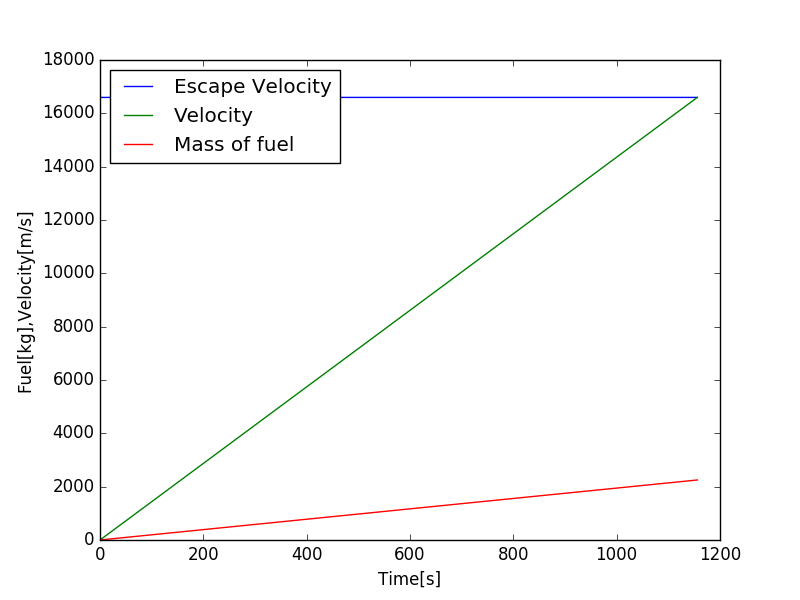
\includegraphics[width = 70mm]{part1launchConstMass.png}
\caption{Shows the mass of fuel increasing has the satellite accelerates. The craft end up using right under 2000 kg of fuel.}
\end{center}
\end{figure}

The plot of the launch with fuel loss shows how the satellite loses fuel as it ascends. The initial fuel was given by equation \ref{eq:Fuel} as $2250.966 kg$.


\begin{figure}[H]
\begin{center}
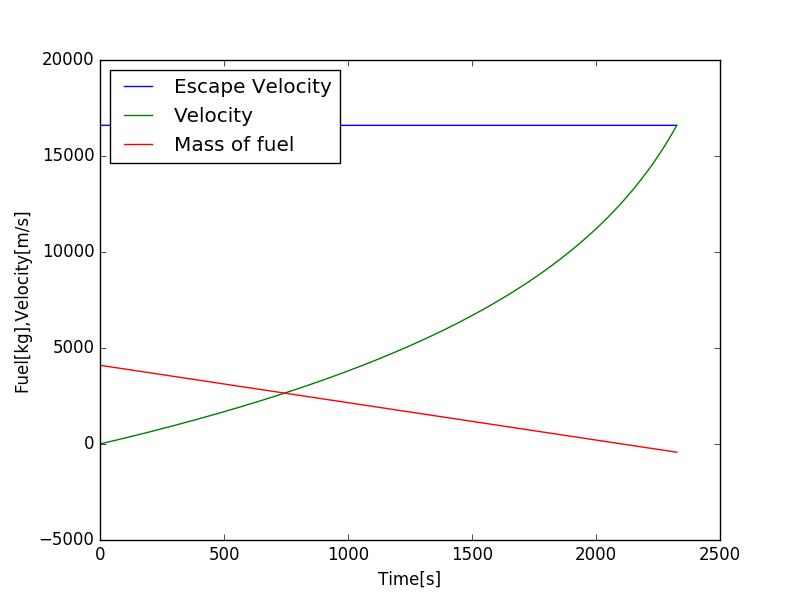
\includegraphics[width = 70mm]{part1launchVarMass.png}
\caption{Shows the mass of fuel slowly going to zeros as the satellite reaches escape velocity.}
\end{center}
\end{figure}

We can see from the plot over that as the satellite reaches escape velocity, the mass of the fuel is more or less zero. This indicates that out expression for fuel gives the correct amount of fuel.

\subsection{Simulation of out Solar System}
\subsubsection{2-body problem}

The first result is with one planet and the sun. We choose to just look at the largest planet and the sun


\begin{figure}[H]
\begin{center}
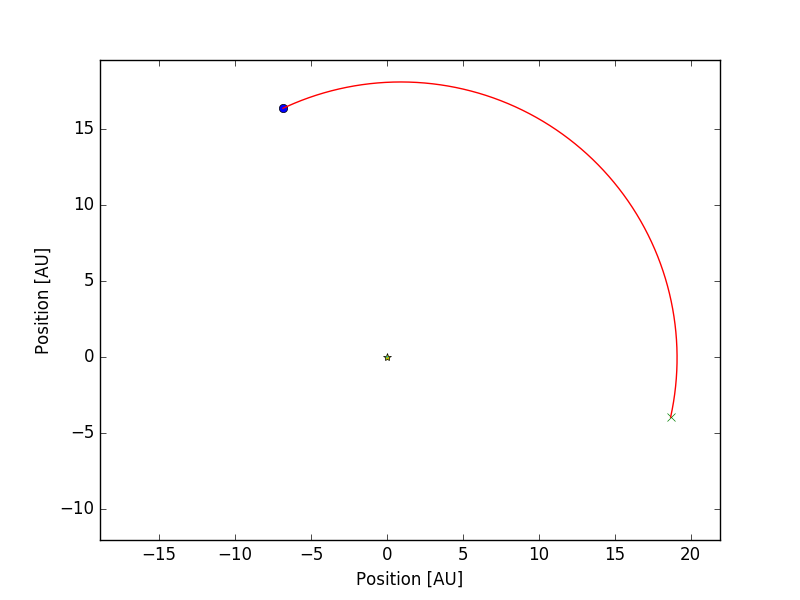
\includegraphics[width = 70mm]{part2onePlanet.png}
\caption{The largest gas giant in the solar system and the sun. Since the planet is quite a distance from the sun, about 16 AU, it only got 1/3 of the way around its orbit during the 20 years.}
\end{center}
\end{figure}

We can see that we have the circular motion we expect, so it passes the rudimentary test for what we expect from planet-sun-system. \\ 

It is more interesting to look at the whole system of 9 planets.

\begin{figure}[H]
\centering
\begin{subfigure}[t]{0.5\textwidth}
\centering
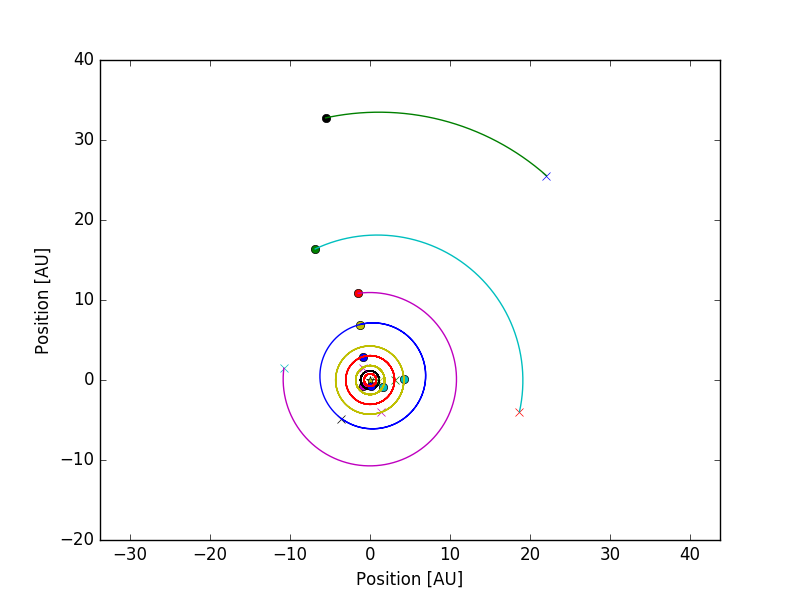
\includegraphics[width=\textwidth]{part2fullSystem.png}
\caption{The orbit of the all 9 planets and the sun. $x$ marks the initial position of the planets, while the ball represents the positions at the end of the simulation.}
\end{subfigure}%
~
\begin{subfigure}[t]{0.5\textwidth}
\centering
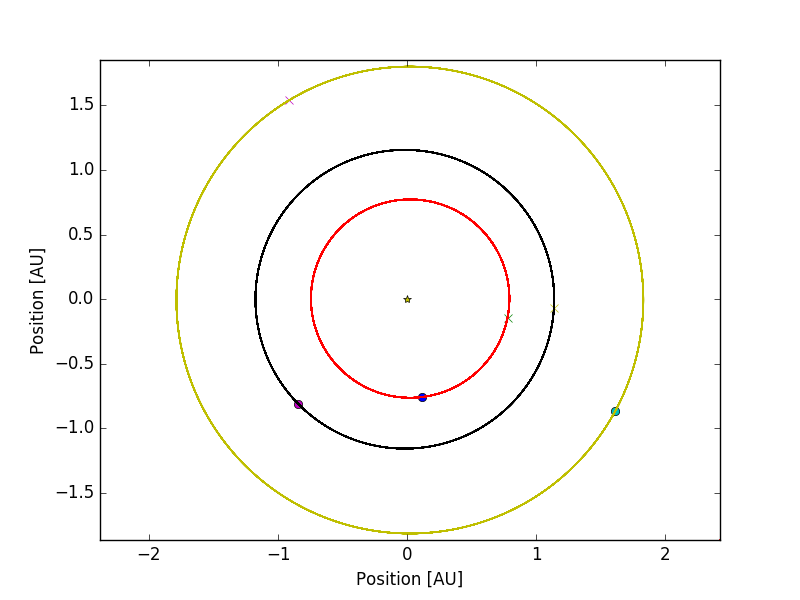
\includegraphics[width=\textwidth]{part2innerPlanets.png}
\caption{A closer look at the inner planets.}
\end{subfigure}%
\end{figure}

We can see that even for the inner planets the simulation seem stable. Since these planets is closer to the sun, they will have orbited more times than the outer planet. There is an error from the numerical method for each orbit, these planets are expected to have accumulated a greater error than the outer planets. Since the we can see that the orbits are stable for the inner planets, we know that the orbits are stable for the rest of the system as well.\\

The orbits were checked against the analytical solutions, and over the 20 year period, the largest relative error was no more than $0.0036\%$.


\subsubsection{N-body problem}
We are interested in seeing how the other planets influence the sun.

\begin{figure}[H]
\begin{center}
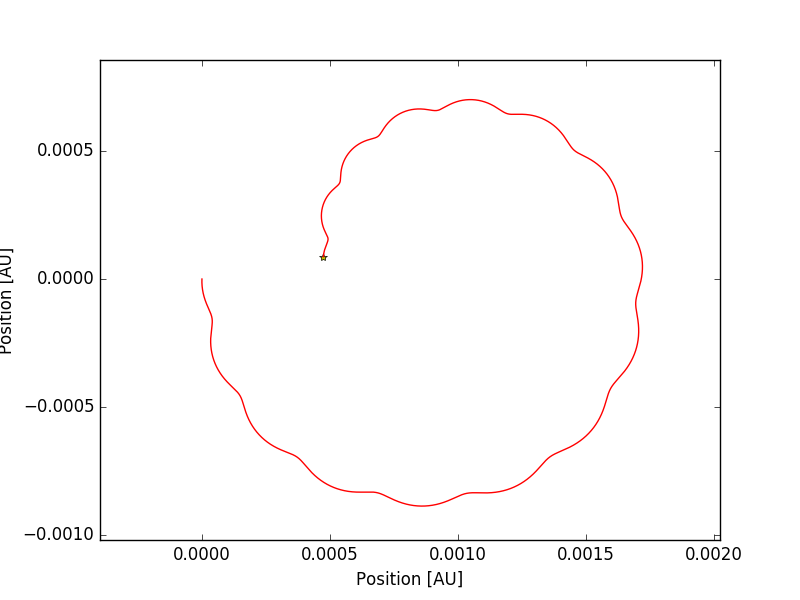
\includegraphics[width = 70mm]{part2posSun.png}
\caption{The motion of the sun. The sun has just finished one orbit of the barycenter of itself and the second largest planet. One can see that this is not a exactly circular orbit, this is because the sun is tugged by the largest planet, which is just 1/4 though its orbit.}
\end{center}
\end{figure}


\begin{figure}[H]
\centering
\begin{subfigure}[t]{0.5\textwidth}
\centering
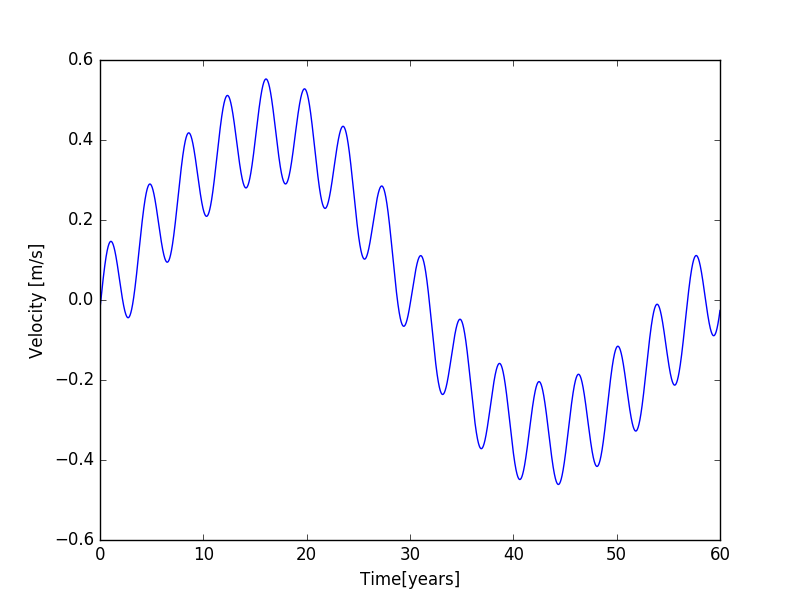
\includegraphics[width=\textwidth]{part2sunNoNoise.png}
\caption{The velocity of the sun towards and away from an observer, gotten from the red shift of the star light.}
\end{subfigure}%
~
\begin{subfigure}[t]{0.5\textwidth}
\centering
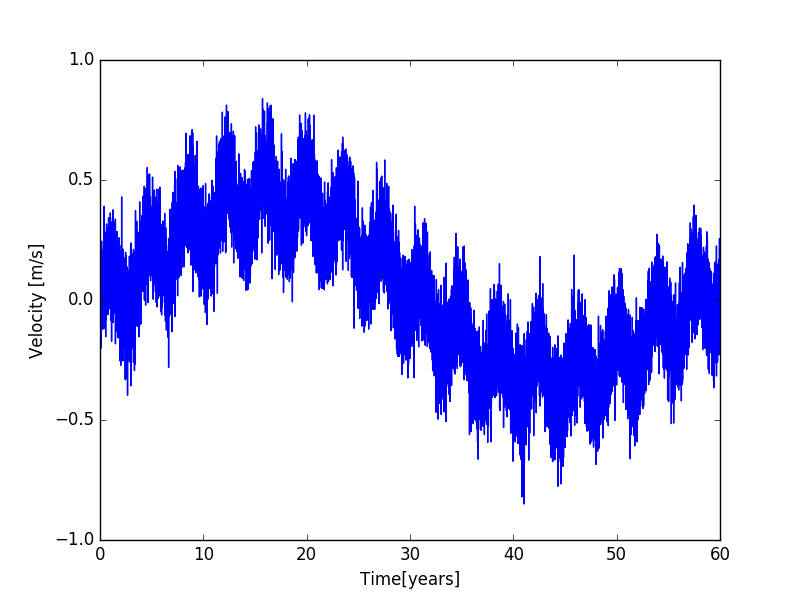
\includegraphics[width=\textwidth]{part2sunNoise.png}
\caption{The velocity of the sun with noise to emulate the noise one gets in real astronomical observations.}
\end{subfigure}%
\end{figure}

We can see that even with noise added to the velocity, the motion is still clearly visible. The difference in velocity is $\pm 0.6 m/s$. With todays technology we are only capable of observing velocity differences of $1 m/s$, meaning that despite there being a clear motion in the data, someone with our technology would not be able to observe it.
















\section{Appendix A: Numerical Methods}
\subsection{Leapfrog}\label{sec:leap}

\subsection{Gradient descend}\label{sec:gradient}

 
\begin{itemize}
\item $F_b$: Force from \textit{one} box.
\item $n_b$: Number of boxes.
\item $m_l$: Mass of the satellite.
\item $m_f$: Mass of the fuel.
\item $m_e$: Mass of the particles escaping per second per box.
\item $m_{f0}$: Mass of fuel when launching.
\end{itemize}

\section{Appendix B: Fuel Equation}\label{sec:Fuel}

To find an analytical expression for the fuel use, we are going to derive the rocket equation using the parameters we get from out engine. We are going to start with Newton's 2. law to find the acceleration for our system:

\begin{equation}
a = \frac{F}{m} = \frac{F_b n_b}{m_f(t) + m_l} 
\end{equation}

Since the system are losing mass:

\begin{equation}
a = \frac{F_b n_b}{(m_{f0} - n_b m_e t) + m_l} = \frac{F_b n_b}{(m_{f0} - \Delta m t) + m_l}
\end{equation} 

Where $m_{f0}$ is the initial mass of the fuel, and $\Delta m$ is the mass loss per second. We separate the variables and solve the differential equation:

\begin{equation}
v(t) = \int \frac{F_b n_b}{(m_{f0} - \Delta m t) + m_l} dt
= K - \frac{F_b}{m_e} \ln(m_{tot} - \Delta m t) 
\end{equation}

Where $m_{tot} = m_l + m_{f0}$. Using the boundary expression we find

\begin{equation}
K = v_0 + \frac{F_b}{m_e} \ln (m_{tot})
\end{equation}

This gives us the rocket equation for our satellite: 

\begin{equation}
v(t) =v_0 + \frac{F_b}{m_e} \ln \left(\frac{m_{tot}}{m_{tot} - \Delta m t} \right)
\end{equation}

We can see that $\frac{F_b}{m_e}$ has the dimension of velocity. This expression corresponds to the velocity of particles escaping (exhaust velocity). If we call this $v_e$ we have the original rocket equation. We want to have use all the fuel when the desired $\Delta v$ i reached. The only mass left then is the mass of the satellite, so $m_{tot} - \Delta m t = m_l$. From this we can find the equation for fuel needed:

\begin{equation}
m_{f0} = m_l(e^{\frac{\Delta v m_e}{F_b}} - 1)
\end{equation}


\section{Appendix C: The Expression for the Atmosphere}\label{sec:atmosphere}
\subsection{The isothermal atmosphere}
To find the analytical expression for the isothermal part of atmosphere we start with the equations for an ideal gas \cite{1e}

\begin{align}\label{eq:idealgas}
P = \frac{\rho kT}{\mu m_H}
\end{align}

and for hydrostatic equilibrium 

\begin{align}\label{eq:hydrostatic}
\frac{dP}{dr} = -\rho \frac{GM(r)}{r^2}
\end{align}

We are going to make the approximation that the gravitational acceleration is the same in the whole atmosphere:

\begin{align}
\frac{GM(r)}{r^2} = g_r
\end{align}

we solve \ref{eq:idealgas} for $\rho$ and sat it in to \ref{eq:hydrostatic}, we get that

\begin{align}
\frac{dP}{dr} = -Pg h_0
\end{align}

\begin{align}
h_0 = \frac{kT}{m_H g \mu}
\end{align}

This differential equation can easily be solved by separating variables, and we get that

\begin{align}
P(h) = C e^{-\frac{h}{h_0}} = P_0 e^{-\frac{h}{h_0}}
\end{align}

And using this in the ideal gas law we find

\begin{align}
\rho (h) = \frac{P_0}{h_0} e^{-\frac{h}{h_0}} = \rho_0 e^{-\frac{h}{h_0}}
\end{align}

\subsection{The adiabatic atmosphere}
Including equations \ref{eq:idealgas} and \ref{eq:hydrostatic} there is one more equation for an adiabatic system

\begin{align}\label{eq:abiabatic}
P^{1-\gamma}T^{\gamma} = constant
\end{align}

$\gamma = 1.4$. We do not know this constant but by differentiating the expression we can get rid of it (this first step was inspired by \cite{adia}, but the rest was done by us)

\begin{align}
\frac{d}{dh}(P^{1-\gamma}T^{\gamma}) = \frac{dP}{dh}(1-\gamma)\left(\frac{T}{P} \right)^{\gamma} + \frac{dT}{dh}\gamma \left(\frac{T}{P} \right)^{\gamma-1} = 0
\end{align}

\begin{align}
\Rightarrow \frac{dP}{P} = \frac{\gamma}{\gamma - 1}\frac{dT}{T}
\end{align}

rewriting the hydrostatic equilibrium we get that

\begin{align}
\frac{dP}{P} = -(g h_0) dh = \frac{\gamma}{\gamma - 1}\frac{dT}{T}
\end{align}

And solving this differential equation gives us the temperature

\begin{align}
T(h) = -g h_0 \frac{\gamma-1}{\gamma}h + C
\end{align}

$T(0) = C = T_0$

\begin{align}\label{eq:adiatemp}
T(h) = T_0 \left( 1 -\frac{\gamma - 1}{\gamma} \frac{h}{h_0} \right)
\end{align}

Setting this back into \ref{eq:abiabatic} we get that

\begin{align}
P(h) = cT(h)^{\frac{\gamma}{\gamma-1}} = cT_0 \left( 1 -\frac{\gamma - 1}{\gamma} \frac{h}{h_0} \right)^{\frac{\gamma}{\gamma-1}} = P_0\left( 1 -\frac{\gamma - 1}{\gamma} \frac{h}{h_0} \right)^{\frac{\gamma}{\gamma-1}}
\end{align}

Now using the ideal gas law we get that

\begin{align}
\rho (h) = \frac{P(h)}{T(h)}\frac{\mu m_H}{k} = \frac{P_0}{T_0}\frac{\mu m_H}{k}\left( 1 -\frac{\gamma - 1}{\gamma} \frac{h}{h_0} \right)^{\frac{\gamma}{\gamma-1} - 1}
\end{align}

\begin{align}\label{eq:adiadens}
\rho (h) = \rho_0 \left(1-\frac{\gamma - 1}{\gamma} \frac{h}{h_0}\right)^{\frac{1}{\gamma - 1}}
\end{align}

\subsection{The boundary}
We are interested in finding $\rho_0$ for the isothermal atmosphere, which is the pressure at the height where $T(h) = T_0/2$. If we use \ref{eq:adiatemp} with  $T(h) = T_0/2$ and solve for $h$, we find that this hight is

\begin{align}
h_{boundary} = \frac{\gamma}{2(\gamma -1)}h_o
\end{align}

and using this in \ref{eq:adiadens} we get that 

\begin{align}
\rho_0^{isothermal} = \rho(h_{boundary}) = \rho_0 \left(\frac{1}{2} \right) ^{\frac{1}{\gamma +1}}
\end{align}


\bibliography{ref} 
\bibliographystyle{plain}






\end{document}